\scanpage{37}\mspage{$\underline{\overline{\mathrm{X}}}$}
\margin{!!}Reste le cas $\mathring{T}\cap\Gamma\ne\unsure{\phi|\varnothing}$. Considerons l'enveloppe convexe\margin{ce n'est pas un ``\unsure{ens.|env.} conv.''!\par
\figure{\begin{tikzpicture}[x=1cm,y=1cm]
\draw[line width=.35pt] (0,0) .. controls (.20,.32) and (.46,.70) .. (.75,.90);
\end{tikzpicture}}} $\unsure{\mathbb{C}|C}$ de $(\mathring{T}\cup\inserted{\bigl[}]s',s''[\inserted{\bigr]})\cap\Gamma$.

On a $\mathbb{C}\subset T-([s,s']\cup[s,s''])$. Observons que $S(\partial C)\deleted{\unsure{\subset|\cap}}\cap\mathring{T}\subset S(\Gamma)$.

Comme $\mathring{T}\cap\Gamma\ne\phi$ il y a\deleted{\illegible{1}} au moins un sommet de $\partial C$ à l'interieur $\mathring{T}$. \unsure{Le|le} lemme $\underline{\overline{\mathrm{IV}}}$ montre qu'il existe $y\notin S(\partial C)$, $y\in\mathbb{C}$, tel que $y$ est $(\mathbb{R}^2-\mathbb{C})$-visible de $s$

(Noter aussi que $\mathring{C}\ne\phi$ puisque $\Gamma\cap\mathring{T}\ne\phi\Rightarrow\operatorname{card}(\Gamma\cap]s',s''[)\geq 2$)

Soit $\alpha\in A(\partial C)$ telle que $y\in\alpha$ le lemme V montre que tout point de $\alpha$ est $(\mathbb{R}^2-C)$-visible de $s$. Si $\alpha=[z,z']$ montrons que $z^{\deleted{\unsure{\prime}}}\notin[s',s'']$ ou bien $z^{\unsure{\prime|\prime\prime}}\notin[s',s'']$. Soit donc $z''\in\mathring{T}\cap\Gamma$ et considerons le triangle $T'$ de sommets $z,z',z''$. Si $z',z''\in[s',s'']$ on voit que $]\unsure{s|S},y[$ ($y\in]z,z'[$) coupe $\mathring{T}'$ selon un ensemble non-vide. Cela contredit le choix de $y$ puisque $\mathring{T}'\subset\mathbb{C}$, \deleted{\unsure{c.a|C.a}} donc $z'$ par exemple vérifie $z'\notin[s',s'']$, $z'\in S'(\Gamma)$ (puisque $z'\in S(\partial\mathbb{C})\cap\mathring{T}$) et le lemme \deleted{\unsure{3|5}} V montre que $z'$ est $(\mathbb{R}^2-\mathbb{C})$-visible de $s$, donc $\operatorname{int}\Gamma$-visible de $s$, c.q-f.d.
% Pencil marginal text is written sideways; its internal order around the long rule remains uncertain at the marked groups.
\margin{compliqué, prendre \unsure{un|le|les} sommet de $\Gamma$ \unsure{$\in$} \deleted{\unsure{$\mathring{T}$|$\alpha$}} \unsure{et} qui est à dist. max. de la droite \deleted{\unsure{$\Delta$}} $(s's'')$\par
\figure{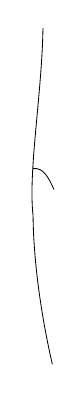
\begin{tikzpicture}[x=.7cm,y=.7cm]
\draw[line width=.3pt] (.42,6.1) .. controls (.40,4.9) and (.15,3.5) .. (.24,2.7) .. controls (.25,1.7) and (.44,.65) .. (.59,0);
\draw[line width=.3pt] (.24,3.55) .. controls (.43,3.58) and (.53,3.37) .. (.62,3.17);
\end{tikzpicture}}}

\uline{Corollaire à la demonstration du lemme $\underline{\overline{\mathrm{VIII}}}$.} \margin{!!}

Si $\Gamma$ est un polygone il existe un couple de sommets \inserted{distincts}\margin{\figure{\begin{tikzpicture}[x=.5cm,y=.5cm]
\draw[line width=.3pt] (-.15,-.95) .. controls (-.35,-.25) and (.10,-.25) .. (1.05,-.20) .. controls (2.1,-.16) and (2.95,.00) .. (3.18,.35);
\end{tikzpicture}}} $s,s'\in S(\Gamma)$ tels que $s'$ est \deleted{\unsure{vis}} $(\mathbb{R}^2-\Gamma)$-visible de $s$ et $]s',s[\subset\partial E(\Gamma)$.
% archive sheet number: 36
